\documentclass{beamer}
\usetheme{metropolis}
\usepackage[utf8]{inputenc}
\usepackage{xcolor}
\usepackage{tikz}


%Information to be included in the title page:
\title{Bayesian Statistics Homework 1}
\subtitle{Gelman et al., \textit{A Weakly Informative Default Prior Distribution For Logistic and Other Regression Models} (2008)}
\author{Roberto Corti}
\date{\today}

\setbeamercolor{background canvas}{bg=white}

\begin{document}
	
	\frame{\titlepage}
	
	\begin{frame}{Logistic regression: \textit{we have some problems}... }
		In some cases, Maximum Likelihood estimates of the coefficients can lead to unstable results.
		
		\begin{figure}
			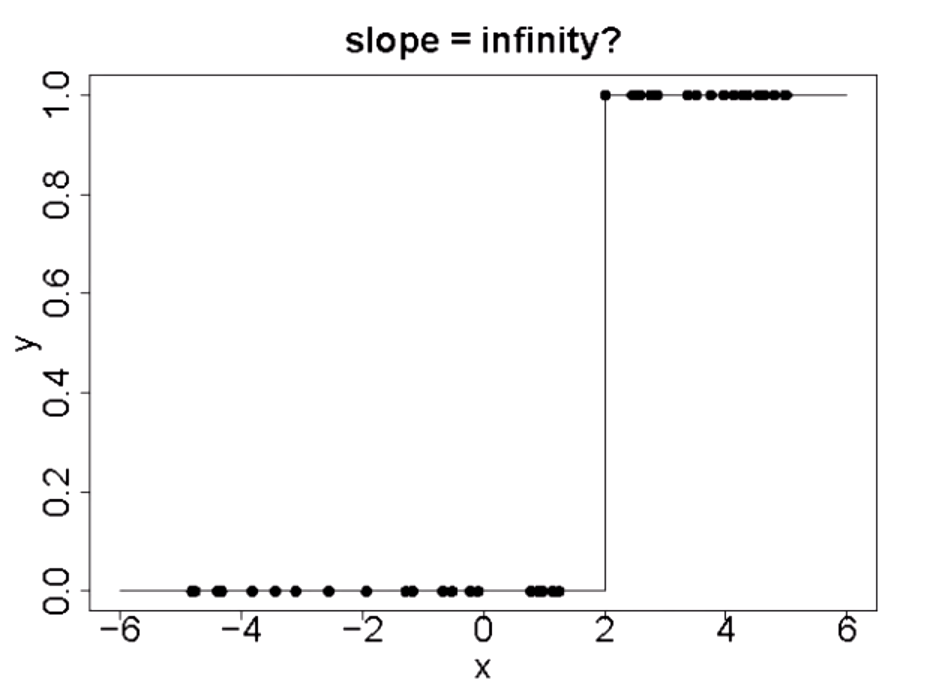
\includegraphics[scale=0.2]{imgs/separation.png}
		\end{figure}
		

		
	\end{frame}
	
\begin{frame}[t]{The need of (weak) prior information}
		
		Adding a prior distribution over regression's coefficient can regularize unstable results.
		\vspace{0.4cm}
		
		Which kind of prior do we use?
		
		\begin{itemize}
			\item Non-informative prior
			\item Fully informative prior
		\end{itemize}
	
		\vspace{0.3cm}
		The aim is to provide \textit{weakly informative priors}
		\begin{itemize}
			\item provide minimal information
			\item able to give regularized coefficient estimates
		\end{itemize}
	
\end{frame}

\begin{frame}{General assumptions for weakly-informative priors}
	
	 What prior information can be assumed for a generic model?
	
	\vspace{0.2cm}
	
	\textit{"For logistic regression, a change of 5 in the logistic scale moves a probability from 0.01 to 0.5, or from 0.5 to 0.99"}
	
	%\vspace{0.2cm}
	
	%Given the logistic regression coefficients $ \beta = (\beta_0, \beta_1, ..., \beta_J ) $ \\
	%if $\beta_i \simeq 5$, for $x=(x_1, ..., x_J) \rightarrow x' =(x_1, ...,x_i+1, ..., x_J)$, then:
	%$$ P(y_i=1 | x)=0.01 \rightarrow P(y'_i=1 | x') \simeq 0.5 $$ 
	
	We rarely encounter this kind of situations, thus  we are willing to assign for $\pi(\beta_i)$ low probabilities for values outside $ [-5, 5]$
	
\end{frame}


\begin{frame}{General assumptions for weakly-informative priors}
	
	In order to have a default prior that could be used in many different contexts, it has to be defined over a commonly interpretable scale.
	
	\vspace{0.4cm}
	It is required to \textit{standardize} the input variables:
	\begin{itemize}
		\item For binary varibales, inputs must have 0 mean and they have to differ 1 in their lower and upper values.
		\item Other variables must have 0 mean and standard deviation of 0.5.
	\end{itemize}
	
\end{frame}

\begin{frame}{General assumptions for weakly-informative priors}
	
	Which probability distribution can be used for this prior?
	
	\vspace{0.2cm}
	
	\begin{itemize}
		\item prior independence: $\pi(\beta) = \pi(\beta_0) \cdot \pi(\beta_1) \cdot ... \cdot \pi(\beta_J)$ 
		\item t-Student family: flat-tailed distributions, easy and stable computations.
	\end{itemize}
	Typical choices can be:
	\begin{itemize}
		\item  for the coefficient terms $\beta_1, ..., \beta_J$, model as a likelihood of a binomial trial with half successes and half failures:  \\
		$\pi(\beta_i) = t_{\nu=1}(\theta=0, s=2.5)$ (Cauchy distribution).
		\vspace{0.3cm}
		\item for the costant term $\beta_0$, allow a success probability between $10^{-9}$ and $1-10^{-9}$ for units
		that are average in all the inputs: \\
		$\pi(\beta_0) = t_{\nu=1}(\theta=0, s=10)$ (Cauchy distribution).
	\end{itemize}
	
\end{frame}



\begin{frame}{A tool to use weakly-informative priors in R}
	
		\centering
		\textbf{\texttt{bayesglm}}\\
		\vspace{0.2cm}
		\begin{itemize}
			\item \textbf{Goal}: \small get MAP estimates $\beta_{MAP}$ and $V_{\beta_{MAP}}$
			\item \textbf{Computation}: \small {Considering the prior distribution for each coefficient as a mixture of normals with unknown scale $\sigma_i$}  $$\pi(\beta_i) = \pi(\beta_i|\sigma_i) \pi(\sigma_i) = \mathcal{N}(\mu_i, \sigma_i^2) \text{inv-}\chi^2(\nu^2_i, s^2_i)$$
			estimates of $\beta_{MAP}$ and $V_{\beta_{MAP}}$ are obtained in a iterative way: \\
			\vspace{0.2cm}
			- for a fixed $\sigma$, approximate the priors as $\pi(\beta_i) \approx \mathcal{N}(\mu_i, \sigma_i^2)$ and get $\hat{\beta}$ by using weighted least squares. \\
			- determine the expected value of the log-posterior density $\log p(\beta, \sigma | X, y)$ and maximize it with respect to $\sigma$ in order to get to get the estimate $\hat{\sigma}$
		\end{itemize}
		
\end{frame}



\begin{frame}{Applications of \texttt{bayesglm} (1)}
	\begin{figure}
		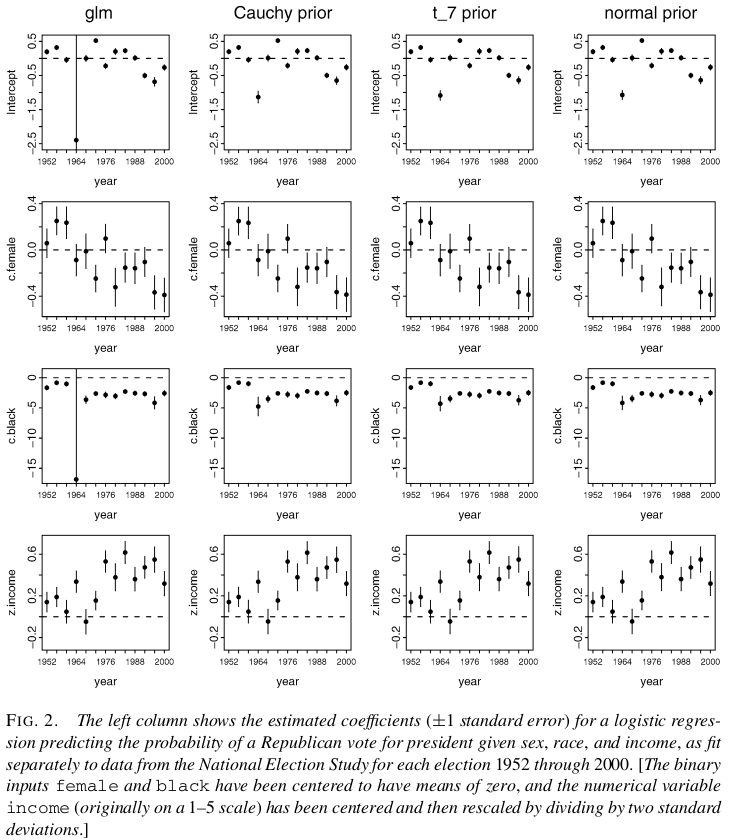
\includegraphics[scale=0.278]{imgs/result1.png}
	\end{figure}
\end{frame}

\begin{frame}{Applications of \texttt{bayesglm} (2)}
	\begin{figure}
		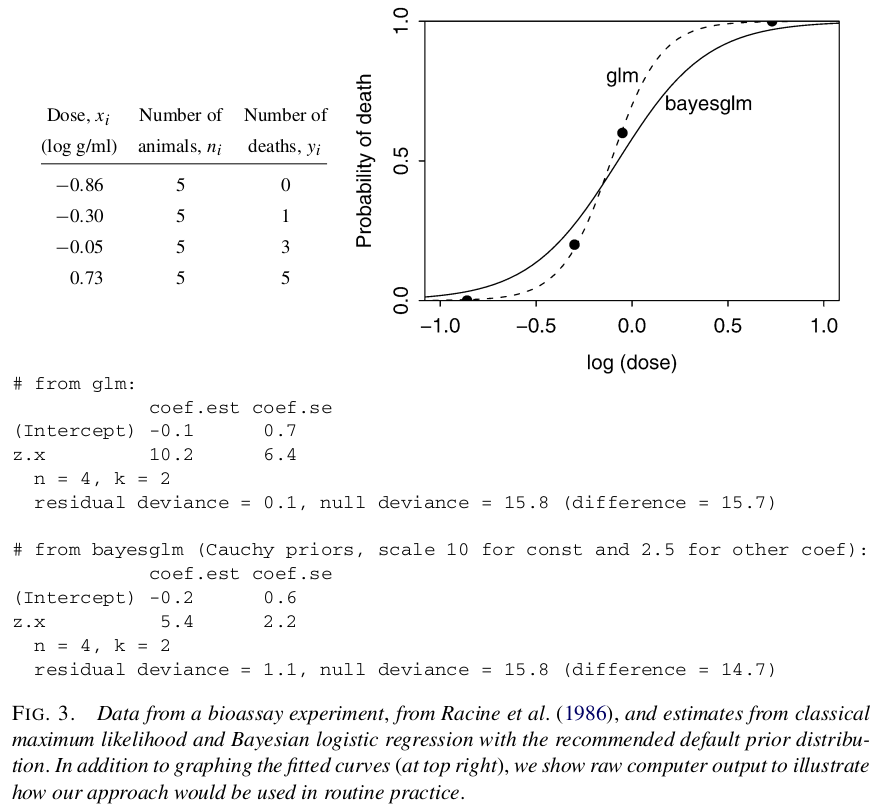
\includegraphics[scale=0.278]{imgs/result2.png}
	\end{figure}
\end{frame}

\begin{frame}{Applications of \texttt{bayesglm} (3)}
	\begin{figure}
		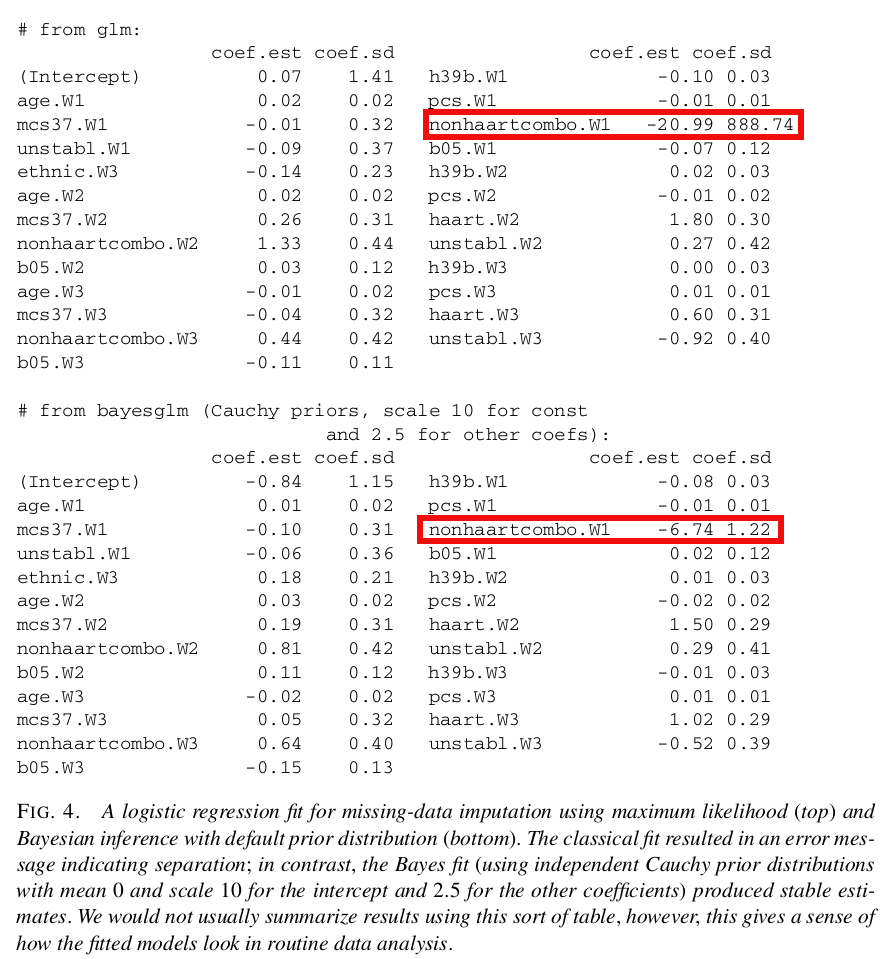
\includegraphics[scale=0.24]{imgs/result3.png}
	\end{figure}
\end{frame}

\begin{frame}{Applications of \texttt{bayesglm} (4)}
	\begin{figure}
		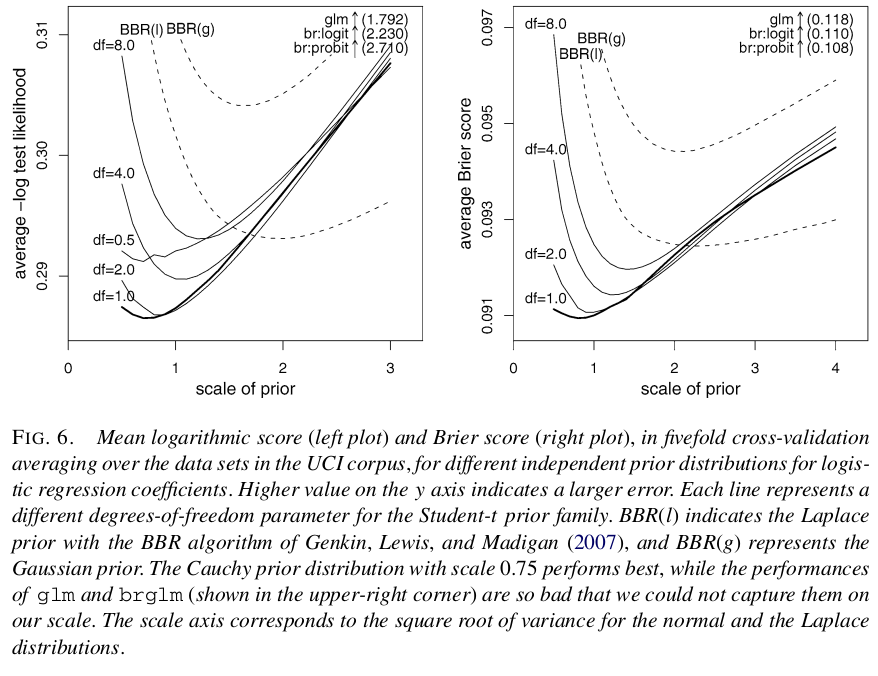
\includegraphics[scale=0.24]{imgs/result4.png}
	\end{figure}
\end{frame}



	
\end{document}